% This file was created with tikzplotlib v0.9.16.
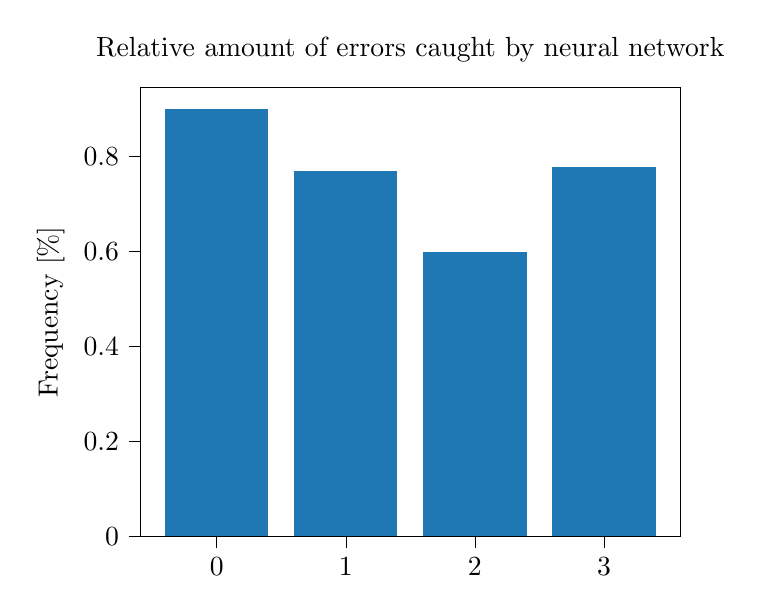
\begin{tikzpicture}

\definecolor{color0}{rgb}{0.12156862745098,0.466666666666667,0.705882352941177}

\begin{axis}[
tick align=outside,
tick pos=left,
title={Relative amount of errors caught by neural network},
x grid style={white!69.0196078431373!black},
xmin=-0.59, xmax=3.59,
xtick style={color=black},
y grid style={white!69.0196078431373!black},
ylabel={Frequency [\%]},
ymin=0, ymax=0.945,
ytick style={color=black}
]
\draw[draw=none,fill=color0] (axis cs:-0.4,0) rectangle (axis cs:0.4,0.9);
\draw[draw=none,fill=color0] (axis cs:0.6,0) rectangle (axis cs:1.4,0.770833333333333);
\draw[draw=none,fill=color0] (axis cs:1.6,0) rectangle (axis cs:2.4,0.6);
\draw[draw=none,fill=color0] (axis cs:2.6,0) rectangle (axis cs:3.4,0.778761061946903);
\end{axis}

\end{tikzpicture}
